\documentclass[answers]{exam}

\usepackage[dvipsnames]{xcolor}
\usepackage{amsmath}
\usepackage{amsfonts}
\usepackage{amsthm}
\usepackage{microtype}
\usepackage{siunitx}
\DeclareSIUnit\year{yr}
\usepackage{pgfplots}
\usepackage{graphicx}
\usepackage{sidecap}
\sidecaptionvpos{figure}{c}
\usepackage{float}
\usepackage{gensymb}
\usepackage{tkz-euclide}
\usetkzobj{all}
\usepackage{commath}

\newtheorem*{thm}{Theorem}

\renewcommand*{\thefootnote}{\fnsymbol{footnote}}

% russian integral
\usepackage{scalerel}
\DeclareMathOperator*{\rint}{\scalerel*{\rotatebox{17}{$\!\int\!$}}{\int}}

% \qformat{Question \thequestion: \thequestiontitle\hfill}

\begin{document}

\section*{NCEA Level 2 Physics, assignment on rotation}


\begin{questions}
  \question I have a rigid vertical rod of length \SI{0.5}{\metre}, pivoted at one end so that
            the other end is free to swing in a circle. I put a mass of \SI{300}{\gram}
            at the free end. This is visualised in the following diagram, where gravity is pointing
            directly down the page.

            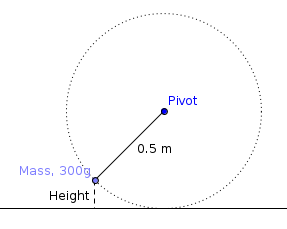
\includegraphics[width=0.4\textwidth]{pendulum}
    \begin{parts}
      \part Suppose that at the instant of time depicted, the pendulum is swinging \emph{down}. On the
            diagram above, draw in \emph{all} the forces acting on the mass. (Hint: there are two!)
      \part The pendulum is pulled up to a height of \SI{0.5}{\metre} (i.e. the pendulum rod is
            horizontal) and then the mass is released. Assuming there is no energy loss due to friction,
            calculate:
        \begin{subparts}
          \item The speed the mass will be travelling around the circle when it reaches the bottom.
          \item The tension force in the rod as the mass reaches the bottom. (What is providing the tension force?)
          \item The maximum height the mass will reach on the other side of its swing.
        \end{subparts}
    \end{parts}
  \question Earth is at a distance \SI{1.496e11}{\metre} from the Sun. It takes one year for the
            earth to complete a single orbit. We will use this information (and only this information!) to calculate the mass of the sun.
    \begin{parts}
      \part A year is 365.25 days; how many seconds is this? (Just work it out to 2 or 3 significant figures.)
      \part Assuming the orbit of the earth is circular, a top-down view looks like this:

            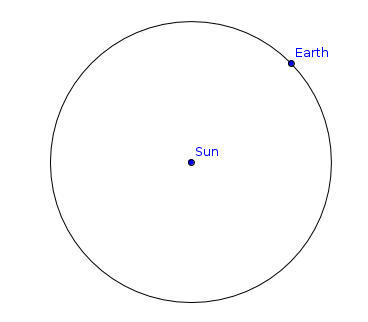
\includegraphics[width=0.4\textwidth]{earth}
        \begin{subparts}
          \item Calculate the circumference of the orbit of the earth.
          \item From (i) we know how far the earth travels each year; from (a) we know how long it takes
                to travel that distance. What is the average speed of the earth around its orbit?
          \item Hence calculate the centripetal acceleration $ a_{\text{centripetal}} $ felt by the earth in orbit.
        \end{subparts}
      \part The centripetal force on the earth is just the gravitational force exerted on the earth by the sun.
            The law of Newtonian gravity tells us that if two objects of mass $ m $ and $ M $ are a distance $ r $
            apart, then the gravitational force between them has magnitude
            \begin{displaymath}
              F_\text{grav} = \frac{GMm}{r^2}
            \end{displaymath}
            where $ G \approx \SI{6.67}{\metre\cubed\per\kilogram\per\second\squared} $ is some constant that is the same everywhere
            in the universe. Let $ m $ be the mass of the earth, and $ M $ be the mass of the Sun. We have
            \begin{displaymath}
              F_{\text{grav}} = F_{\text{centripetal}} \implies \frac{GMm}{r^2} = m a_\text{centripetal}.
            \end{displaymath}
            Note that the mass $ m $ of the earth cancels from both sides. Using your value of $ a_\text{centripetal} $ from (b)
            above, substitute everything in and work out the value of $ M $.\footnote{You should get something like \SI{1.99e30}{\kilo\gram}.}
    \end{parts}
  \question A child (at school on Earth, so they feel gravity) swings a ball on a string in a horizontal circle around their head, in
            such a way that the speed of the ball around the circle is constant. Nothing else is touching the ball.
    \begin{parts}
      \part State, with \emph{detailed} reasoning, whether the following statement is true or false.

            \emph{The ball is moving at a constant speed, so it is not accelerating.}

      \part Explain why the string can \emph{never} be horizontal in this situation, no matter how fast the ball is swung or how tightly
            the child is gripping the string. (You may find it useful to draw the forces acting on the ball.)
    \end{parts}
  \question Two children, of masses \SI{50}{\kilo\gram} and \SI{55}{\kilo\gram}, sit opposite each other on a see-saw so that it is exactly
            balanced. The pivot is at the middle of the see-saw.
    \begin{parts}
      \part We don't know the mass of the see-saw. However, this doesn't matter: the torque around the pivot due to the force
            of gravity on the see-saw is zero. Why?
      \part The lighter child is sitting right at the end of the see-saw. What distance is each child sitting from the pivot?
      \part The heavier child now moves so that they are sitting right at the end of the see-saw, so that the end of the see-saw rests on
            the ground.
        \begin{subparts}
          \subpart Explain why the mass of the see-saw still doesn't matter to us: it still contributes no torque about the axis.
          \subpart What is the force exerted on the ground at the end of the see-saw resting on the ground?
        \end{subparts}
    \end{parts}
\end{questions}


\end{document}
